\subsection{Módulos y componentes}

\subsubsection{STM32 Nucleo-144}


La STM32 Nucleo-144 es una placa de desarrollo basada en los microcontroladores STM32 de la familia ARM Cortex-M, diseñada para facilitar la creación de prototipos y el desarrollo de sistemas embebidos \cite{nucleo144}. Esta placa es parte de la serie Nucleo de STMicroelectronics, conocida por ofrecer soluciones flexibles y accesibles para una amplia gama de aplicaciones, desde dispositivos IoT (\textit{Internet of Things}) hasta sistemas críticos. En la figura \ref{fig:nucleo144} se puede visualizar la placa de desarrollo.\\


\begin{figure}[H]
    \centering
    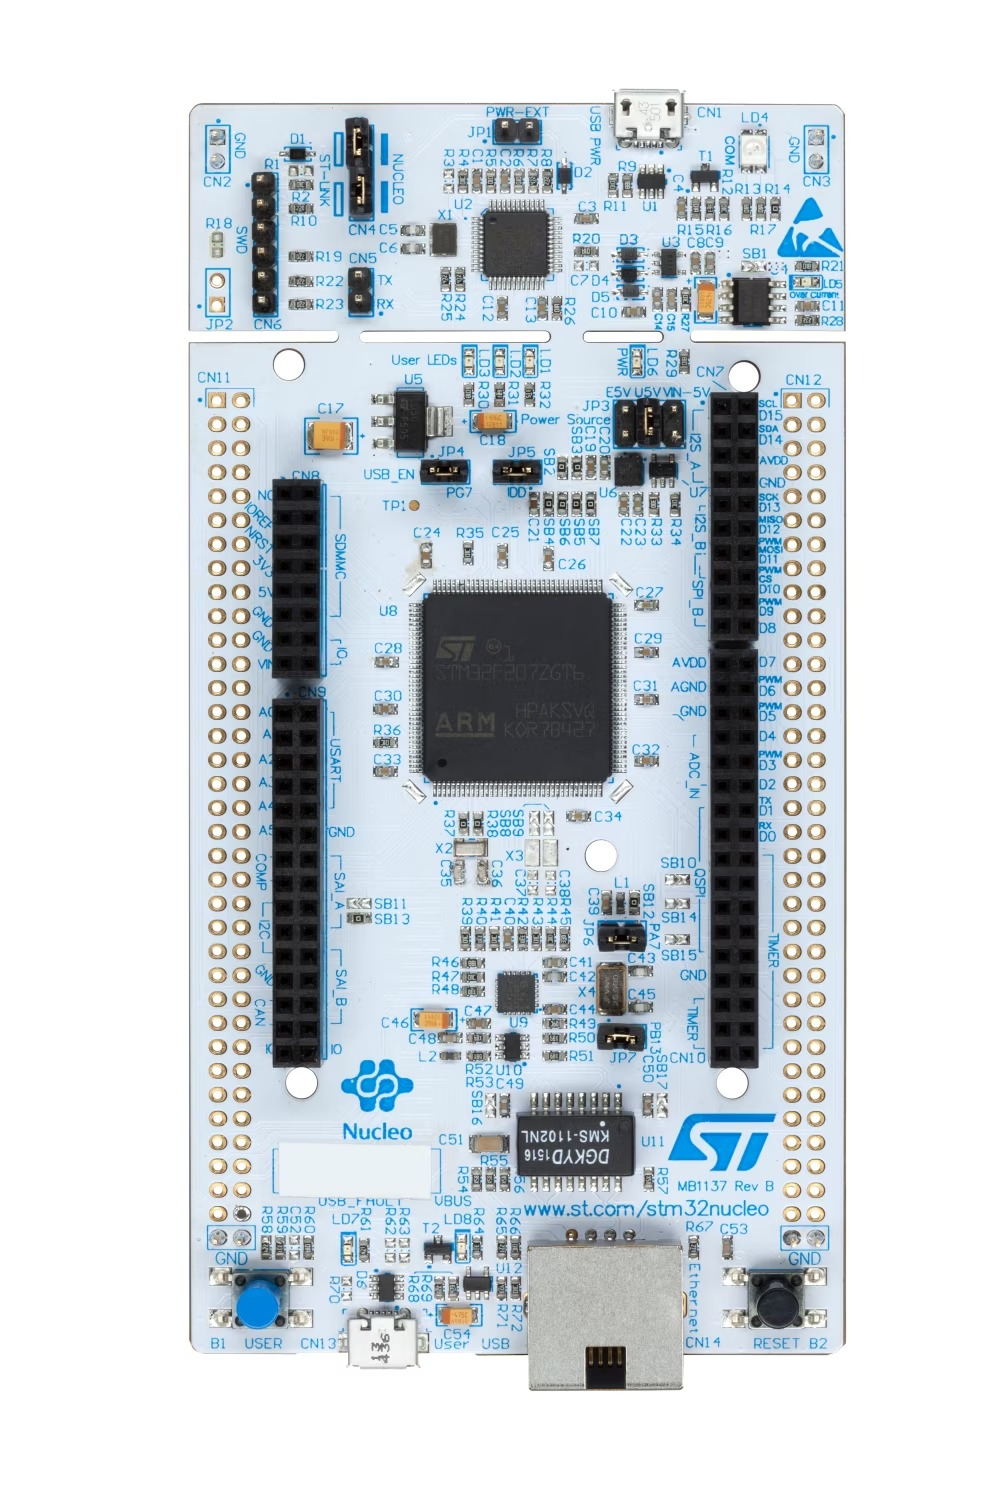
\includegraphics[height=\linewidth, angle=90]{img/nucleo144.jpeg}
    \caption{STM32 Nucleo-144 con microcontrolador STM32F429ZI}
    \label{fig:nucleo144}
\end{figure}



La STM32 Nucleo-144 se caracteriza por su gran versatilidad y un conjunto de características técnicas que la hacen adecuada para proyectos que requieren un rendimiento alto y conectividad avanzada. Entre sus especificaciones más destacadas se incluyen:

\begin{itemize}
    \item \textbf{Microcontrolador}: Está equipada con un microcontrolador basado en la arquitectura ARM Cortex-M que puede variar según el modelo. Estos ofrecen un excelente rendimiento junto con una amplia gama de interfaces de conectividad y capacidades avanzadas de procesamiento en tiempo real. Particularmente, la versión que incluye el microcontrolador STM32F429ZI \cite{stm32f429zi} tiene un núcleo ARM Cortex-M4 que corre ST-LINK/V2-1a 180 MHz con unidad de punto flotante (FPU), memoria flash de 2 MB y RAM de 256 KB. 
    \item \textbf{Conectividad}: La Nucleo-144 dispone de múltiples interfaces de comunicación, como UART, I2C, SPI, USB, Ethernet y CAN, lo que la convierte en una opción idónea para sistemas que requieren interconexión de múltiples dispositivos y la transmisión de datos en tiempo real.
    \item \textbf{Compatibilidad con \textit{shields} de Arduino}: La placa ofrece conectores que permiten la compatibilidad con los \textit{shields} de Arduino, lo que facilita la ampliación del sistema con componentes adicionales, como sensores o módulos de comunicación, sin necesidad de diseñar hardware personalizado.
    \item \textbf{Pines}: A diferencia de las versiones más compactas, la Nucleo-144 incluye un conector de 144 pines, lo que ofrece una gran cantidad de líneas de entrada/salida (GPIO) para controlar y conectar diversos módulos y periféricos. Además, esto permite acceso a todos los pines del microcontrolador lo que permite mayor flexibilidad para la asignación de sus funciones.
    \item \textbf{Programación integrada y \textit{debugging}}: Incorpora una interfaz ST-LINK/V2-1 que permite la programación y depuración del microcontrolador sin necesidad de hardware adicional \cite{st_link}. Esto simplifica el desarrollo y facilita la identificación y corrección de errores durante las pruebas del sistema.
    \item \textbf{Alimentación}: La placa puede ser alimentada tanto por USB como por una fuente externa de 5 V o 3.3 V, lo que la hace adaptable a diferentes entornos operativos.
\end{itemize}

Una de las grandes ventajas de la Nucleo-144 es la posibilidad de desarrollar firmware utilizando herramientas accesibles como STM32CubeIDE \cite{stCubeIde}, que proporciona un entorno de desarrollo completo y gratuito. Mediante una interfaz gráfica, se puede configurar la función de cada uno de los pines, nombrarlos y asegurarse que no haya superposiciones de definiciones o protocolos de comunicación definidos sin los pines necesarios para que funcione. También facilita la configuración de un sistema operativo en tiempo real permitiendo la declaración de las distintas tareas y mecanismos de sincronización. Además, el uso de bibliotecas como STM32CubeMX \cite{stCubeMx} facilita la configuración de los periféricos del microcontrolador y la generación de código, reduciendo el tiempo de desarrollo y minimizando la posibilidad de errores. 


